\section{Une faille csrf: kézako ?}

\frame{\tableofcontents[currentsection]}

\begin{frame}

\begin{itemize}
	\item CSRF: Cross Site Request Forgery ou ("Sea surf")
	\item Rediriger un utilisateur authentifié (admin, user lambda) sur une action interne d'un site.
	\item A pour effet d'exécuter une action avec les privilèges d'un autre utilisateur.
	\item Avantages: très facile de créer des exploit et de les utiliser.
\end{itemize}

\end{frame}

\begin{frame}

\centerline{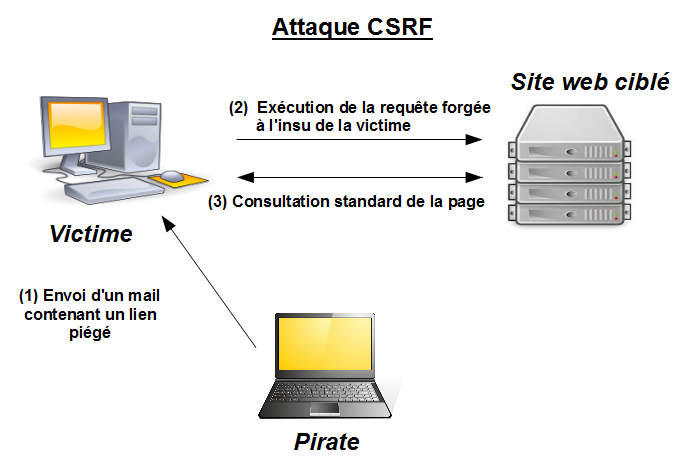
\includegraphics[scale=0.45]{csrf.png}}

\end{frame}